\newpage
\chapter{Platform} \textit{Dennis}
\section{Environment}
The system is primarily to be used from the same PC, as the webpage is part of an energy system
placed at the school, AU Herning. A part of the energy system is a screen showing the webpage to
be able to control the system nearby it. The screens resolution is 1024x768 pixels (fullscreen with no system bars or dock), 
which is the size the site has been optimized for. Also the website has been optimized for small-screen devises with a resolution from 320x480 pixels (as this resolution has been used for several phones in the last years).
\section{File Structure}
The website can be found on http://www.ehub.threee.dk/, the file structure on the ftp server is as follow. In the index folder/root of the site, the folders: Design, Images, Mobile and Scripts can be found together with the different .html files and .css files created for the site. The root folder contains:
\begin{itemize}
	\item Design: Photoshop files
	\item Images: Icons and other pictures used on the site.
	\item Scripts: Java-scripts for further use.
	\item Mobile: .html, .css and images used for the mobile site
	\item .html files (index, hub, wind, etc.)
	\item .css files (style\_index, style\_hub, etc.)
\end{itemize}
\begin{figure}[htbp]
	\center
	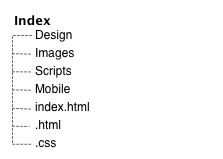
\includegraphics[width=0.25\textwidth]{images/hierarki.png} % requires the graphic package
   	\caption{Hierarki of the files}
   	\label{fig:file_hierarki}
\end{figure}
\newpage
\section{Image scaling}
All images putted on the webpage is scaled in Photoshop using the 'Save for web \& Devices' command. The images are saved as PNG-24 format.

\section{Reset.css} \textit{Theis}\\
The reset css file is used to make default settings for all common stuff. The point of this file is to define the layout for html tags that may not be set up in the other css files. For example that could be a headings tag that looks fine by default, the problem now is that Mozilla Firefox can have one default setting for the headings when Google Chrome maybe have a different default settings for the same headings, this will make the same code look different in the two browsers. The reset css file then defines some default settings for the most common html tags.
